\documentclass[11pt, a4paper]{article}
\usepackage[utf8]{inputenc}
\usepackage[T1]{fontenc}
\usepackage[charter]{mathdesign} % Elegant, readable font
\usepackage{geometry}
\geometry{margin=1in}
\usepackage{enumitem}
\usepackage{amsmath}
\usepackage{booktabs}
\usepackage{hyperref}
\usepackage{graphicx} % Required for inserting images (put this in your preamble)
\usepackage{subfig}


\makeatletter
\renewcommand{\maketitle}{
  \begin{flushleft}
    {\huge \textbf{\@title} \par}
    \vspace{0.5cm}
    {\large \@author \par}
    \vspace{0.2cm}
    {\@date \par}
    \vspace{0.2cm}
    \hrule
  \end{flushleft}
}
\makeatother

\title{\LARGE\textbf{Assignment 2: Lenia — An Artificial Life} \\[-0.2em]
    \large Assignment 1 --- High Performance Computing}
\author{
    Plabon Shaha and Guillem Masdemont \\ 
    \small University of Ljubljana, Spring Semester, EMAI Cohort 25--27 
}

\begin{document}

\maketitle

\begin{enumerate}[label={\textbf{Exercise \arabic*:}}]
  \item We parallelize the algorithm as efficient as we can, and we compare with the base sequential performance with differennt numbers of tiles. The results are averaged over $5$ experiments across diferent resolutions. 

\begin{figure}[htbp]
    \centering
    % Adjust the width if needed (e.g., 0.9\textwidth or \linewidth)
    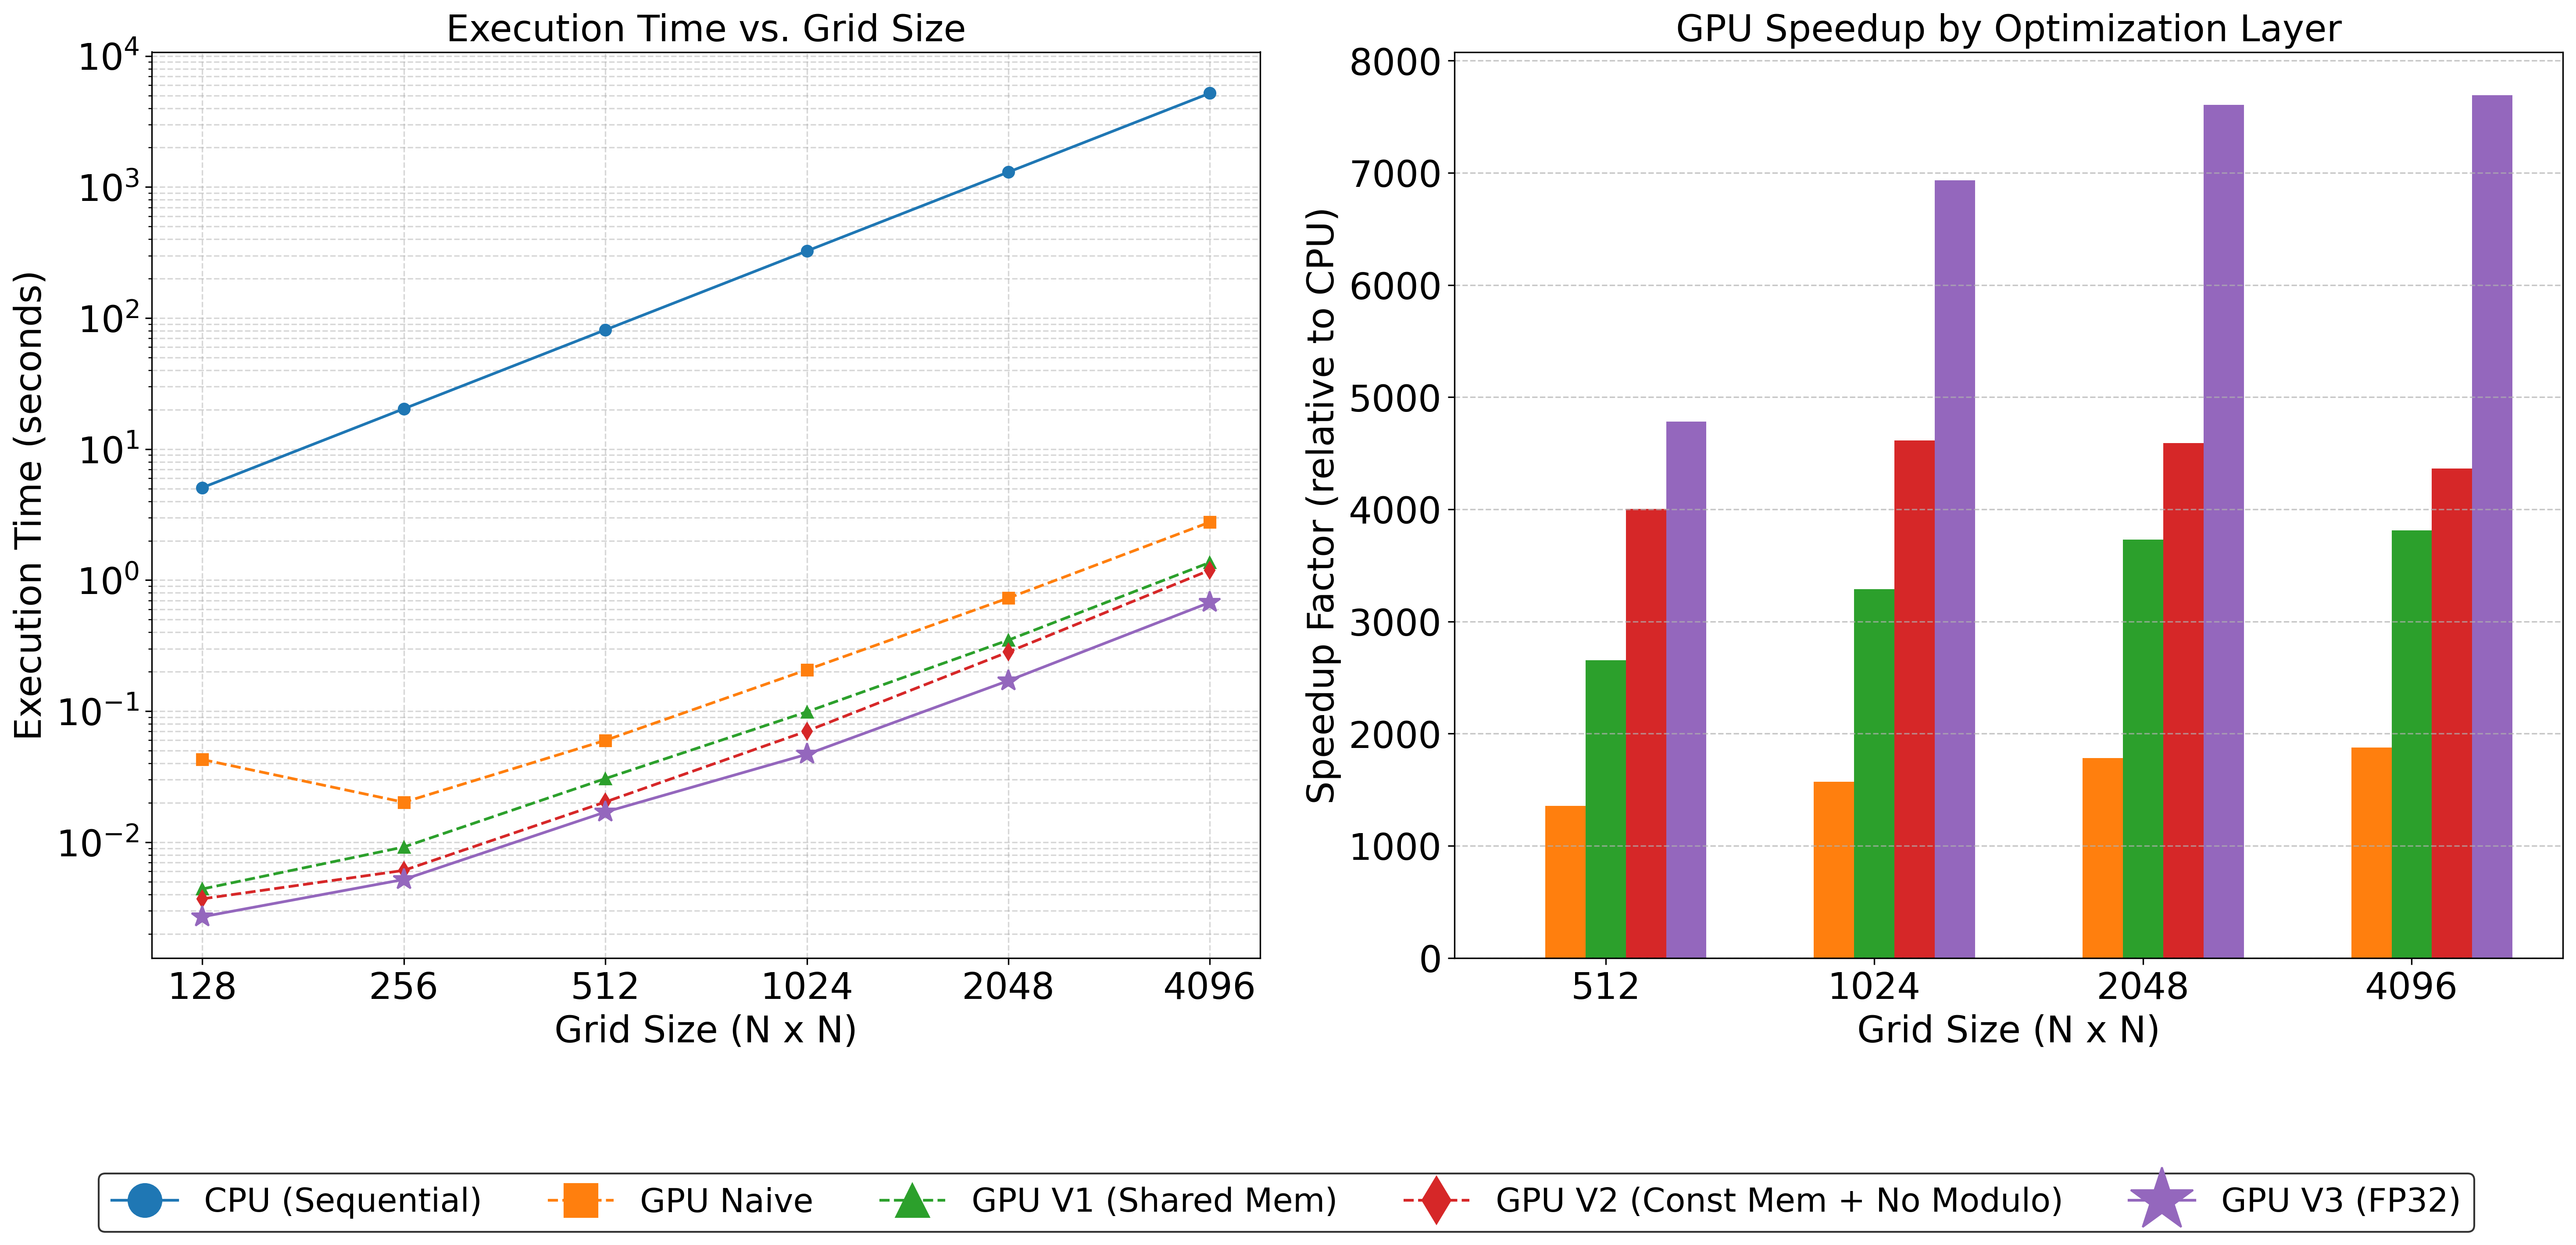
\includegraphics[width=\textwidth]{combined_performance_plots.png}
    \caption{Performance comparison of CUDA optimization layers. \textbf{Left:} Log-log plot showing execution time versus grid size, highlighting the algebraic scaling advantage of the GPU implementations. \textbf{Right:} Grouped bar chart detailing the speedup factor of each GPU kernel relative to the sequential CPU baseline for large grid sizes.}
    \label{fig:performance_plots}
\end{figure}


  \begin{table}[h]
\centering
\caption{Performance Metrics for Tile Size 8}
\begin{tabular}{rcccccc}
\hline
$N$ & $T_{seq}$ & $T_{naive}$ & $T_{v1}$ & $T_{v2}$ & $T_{v3}(f)$ & Speedup($v3$) \\
\hline
128  & 5.0847 & 0.0434 & 0.0048 & 0.0040 & 0.0031 & 1643.31 \\
256  & 20.3207 & 0.0204 & 0.0119 & 0.0094 & 0.0078 & 2591.90 \\
512  & 81.3130 & 0.0603 & 0.0417 & 0.0313 & 0.0275 & 2952.69 \\
1024 & 325.2871 & 0.2123 & 0.1434 & 0.0962 & 0.0882 & 3688.49 \\
2048 & 1301.3061 & 0.7389 & 0.5016 & 0.3584 & 0.3278 & 3969.52 \\
4096 & 5205.5831 & 2.7600 & 1.9797 & 1.4209 & 1.3006 & 4002.36 \\
\hline
\end{tabular}
\end{table}

\begin{table}[h]
\centering
\caption{Performance Metrics for Tile Size 16}
\begin{tabular}{rcccccc}
\hline
$N$ & $T_{seq}$ & $T_{naive}$ & $T_{v1}$ & $T_{v2}$ & $T_{v3}(f)$ & Speedup($v3$) \\
\hline
128  & 5.0795 & 0.0428 & 0.0044 & 0.0037 & 0.0027 & 1886.26 \\
256  & 20.3176 & 0.0202 & 0.0092 & 0.0061 & 0.0052 & 3876.76 \\
512  & 81.2717 & 0.0599 & 0.0306 & 0.0203 & 0.0170 & 4778.02 \\
1024 & 325.1207 & 0.2071 & 0.0989 & 0.0705 & 0.0469 & 6926.76 \\
2048 & 1300.6583 & 0.7305 & 0.3488 & 0.2833 & 0.1710 & 7607.37 \\
4096 & 5203.7136 & 2.7718 & 1.3655 & 1.1927 & 0.6765 & 7692.49 \\
\hline
\end{tabular}
\end{table}

\begin{table}[h]
\centering
\caption{Performance Metrics for Tile Size 32}
\begin{tabular}{rcccccc}
\hline
$N$ & $T_{seq}$ & $T_{naive}$ & $T_{v1}$ & $T_{v2}$ & $T_{v3}(f)$ & Speedup($v3$) \\
\hline
128  & 5.1617 & 0.0426 & 0.0044 & 0.0037 & 0.0027 & 1907.48 \\
256  & 20.3258 & 0.0213 & 0.0094 & 0.0063 & 0.0053 & 3821.09 \\
512  & 81.2846 & 0.0607 & 0.0313 & 0.0199 & 0.0173 & 4711.18 \\
1024 & 325.0540 & 0.2140 & 0.1006 & 0.0732 & 0.0497 & 6537.52 \\
2048 & 1300.5371 & 0.7232 & 0.3510 & 0.2907 & 0.1763 & 7375.32 \\
4096 & 5205.6769 & 2.7460 & 1.3746 & 1.2213 & 0.6974 & 7464.71 \\
\hline
\end{tabular}
\end{table}

The staggered implementation of CUDA optimizations resulted in a peak speedup of nearly $7700\times$ over the sequential CPU baseline. The impact of each architectural consideration can be summarized as follows:

\begin{itemize}
    \item \textbf{Tile Size Optimization ($16 \times 16$ Sweet Spot):} A block dimension of $16 \times 16$ yielded the highest throughput for large grids. Tile size 8 underutilizes the Streaming Multiprocessors (SMs) by spawning too many lightweight blocks, while tile size 32 requires excessive shared memory per block, lowering overall warp occupancy.
    \item \textbf{Shared Memory Tiling ($V1$):} Introducing collaborative loading into \texttt{\_\_shared\_\_} memory eliminated redundant global memory fetches. This optimization alone halved the execution time across almost all grid sizes, proving memory bandwidth to be the primary bottleneck in the naive implementation.
    \item \textbf{Constant Memory and Divergence Reduction ($V2$):} Relocating the convolution matrix to \texttt{\_\_constant\_\_} memory leveraged hardware broadcasting, allowing all threads in a warp to access kernel weights simultaneously. Furthermore, replacing the expensive modulo (\texttt{\%}) wrap-around math with simple bounds checking (\texttt{if/else}) significantly reduced arithmetic latency.
    \item \textbf{Single Precision Floating Point ($V3$):} The transition from 64-bit \texttt{double} to 32-bit \texttt{float} provided an additional $2\times$ performance jump. This effectively doubled the available memory bandwidth and unlocked the massively parallel FP32 cores dominant in consumer-grade GPU architectures.
    \item \textbf{Hardware Saturation:} At smaller grid sizes (e.g., $N=128$), the performance delta between optimizations is minimal. The hardware only becomes fully saturated—revealing the true architectural benefits of the optimization stack—at $N \ge 1024$, where warp scheduling efficiently hides memory latency.
\end{itemize}


\end{enumerate}

\end{document}